\section{Bias and Variance of the Elastic Net Estimator}\label{sec:theory}

% TODO: write a table of the bias and variance formulations for each type instead.

Now, assume that \(\mat{X}\) is fixed and that \(\vec{y} = \mat{X}\vec{\beta} + \vec{\varepsilon}\), where \(\varepsilon_i\) is identically and independently distributed noise with mean zero and finite variance \(\sigma_\varepsilon^2\). As in the previous section, we assume that the feature vectors are orthogonal. We are interested in the expected value of \Cref{eq:orthogonal-solution}, \(\E \hat{\beta}_j\). Let
\[
  Z = \tilde{\vec{x}}_j^\T \vec{y} = \tilde{\vec{x}}_j^\T(\mat{X}\vec{\beta}^* + \vec{\varepsilon}) = \tilde{\vec{x}}_j^\T (\vec{x}_j\beta_j^* + \boldsymbol{\varepsilon})
  \qquad
  \text{and}
  \qquad
  d_j = s_j(\tilde{\vec{x}}_j^\T \tilde{\vec{x}}_j + \lambda_2)
\]
so that \(\hat{\beta}_j = \st_{\lambda_1}(Z)/d_j\). Since \(d_j\) is fixed under our assumptions, we will direct most of our focus towards \(S_{\lambda_1}(Z)\). First observe that
\[
  \begin{aligned}
    \tilde{\vec{x}}_j^\T \tilde{\vec{x}}_j & = \frac{1}{s_j^2}(\vec{x}_j - c_j)^\T (\vec{x}_j - c_j) = \frac{\vec{x}_j^\T\vec{x}_j - nc_j^2}{s^2_j} = \frac{n v_j}{s_j^2}, \\
    \tilde{\vec{x}}_j^\T \vec{x}_j         & = \frac{1}{s_j}(\vec{x}_j^\T \vec{x}_j - \vec{x}_j^\T \ones c_j) = \frac{n v_j}{s_j},
  \end{aligned}
\]
where \(v_j\) is the uncorrected sample variance of \(\vec{x}_j\). This means that
\begin{equation}
  \label{eq:z-d}
  Z = \frac{\beta_j^* n v_j- \vec{x}_j^\T \vec{\varepsilon}}{s_j}
  \qquad\text{and}\qquad
  d_j = s_j\left(\frac{n v_j}{s_j^2} + \lambda_2\right).
\end{equation}
For the expected value and variance of \(Z\) we then have
\begin{align*}
  \E Z   & = \mu = \E \left( \tilde{\vec{x}}_j^\T (\vec{x}_j\beta_j + \vec{\varepsilon}) \right)  = \tilde{\vec{x}}_j^\T\vec{x}_j \beta_j,      \\
  \var Z & = \sigma^2 = \var\left(\tilde{\vec{x}}_j ^\T \vec{\varepsilon}\right) = \tilde{\vec{x}}_j^\T \tilde{\vec{x}}_j\sigma_\varepsilon^2 .
\end{align*}

The expected value of the soft-thresholding estimator is
\begin{align*}
  \label{eq:st-expected-value}
  \E \st_\lambda(Z) & = \int_{-\infty}^\infty \st_\lambda(z) f_Z(z) \du z                                                   \nonumber \\
                    & = \int_{-\infty}^\infty \ind{|z| > \lambda} (z -\sign(z)\lambda) f_Z(z) \du z                         \nonumber \\
                    & = \int_{-\infty}^{-\lambda}(z + \lambda)f_Z(z) \du z + \int_{\lambda}^\infty (z - \lambda)f_Z(z) \du z.
\end{align*}
And then the bias of \(\hat\beta_j\) with respect to the true coefficient \(\beta_j^*\) is
\begin{equation*}
  \label{eq:betahat-bias}
  \E \hat\beta_j - \beta_j^* = \frac{1}{d_j}\E \st_\lambda(Z) - \beta^*_j.
\end{equation*}

Finally, we note that the variance of the soft-thresholding estimator is
\begin{equation}
  \label{eq:st-variance}
  \var {S_\lambda(Z)} = \int_{-\infty}^{-\lambda}(z + \lambda)^2f_Z(z) \du z + \int_{\lambda}^\infty (z - \lambda)^2 f_Z(z) \du z - \left(\E \st_\lambda(Z)\right)^2
\end{equation}
and that the variance of the elastic net estimator is therefore
\begin{equation}
  \label{eq:betahat-variance}
  \var \hat\beta_j = \frac{1}{d_j^2} \var \st_\lambda(Z).
\end{equation}

\subsection{Normally Distributed Noise}

Next, we add the additional assumption that \(\vec{\varepsilon}\) is normally distributed. Then
\[
  Z \sim \normal\left(\mu = \tilde{\vec{x}}_j^\T\vec{x}_j \beta_j, \sigma^2 = \tilde{\vec{x}}_j^\T\tilde{\vec{x}}_j \sigma_\varepsilon^2 \right).
\]
Let \(\theta = -\mu -\lambda_1 \) and \(\gamma = \mu - \lambda_1\). Then the expected value of soft-thresholding of \(Z\) is
\begin{align}
  \E \st_{\lambda_1}(Z) & = \int_{-\infty}^\frac{\theta}{\sigma} (\sigma u - \theta) \pdf(u) \du u + \int_{-\frac{\gamma}{\sigma}}^\infty (\sigma u + \gamma) \pdf(u) \du u                                               \nonumber                      \\
                        & = -\theta \cdf\left(\frac{\theta}{\sigma}\right) - \sigma \pdf\left(\frac{\theta}{\sigma}\right) + \gamma \cdf\left(\frac{\gamma}{\sigma}\right) + \sigma \pdf\left(\frac{\gamma}{\sigma}\right) \label{eq:mean-centered-eval}
\end{align}
where \(\pdf(u)\) and \(\cdf(u)\) are the probability density and cumulative distribution functions of the standard normal distribution, respectively.

Next, we consider what the variance of the elastic net estimator looks like.
Starting with the first term on the left-hand side of \Cref{eq:st-variance}, we have
\begin{align}
  \label{eq:mc-var-part1}
  \int_{-\infty}^{-\lambda_1}(z+ \lambda_1)^2 f_Z(z) \du z & = \sigma^2 \int_{-\infty}^{\frac{\theta}{\sigma}} y^2 \pdf(y) \du y + 2 \theta \sigma \int_{-\infty}^{\frac{\theta}{\sigma}} y \pdf(y) \du y + \theta^2 \int_{-\infty}^{\frac{\theta}{\sigma}} \pdf(y) \du y                                                                               \nonumber \\
                                                           & = \frac{\sigma^2}{2} \left( \erf\left(\frac{\theta}{\sigma\sqrt{2}}\right) - \frac{\theta}{\sigma}\sqrt{\frac{2}{\pi}} \exp\left(-\frac{\theta^2}{2\sigma^2}\right) + 1 \right) + 2 \theta \sigma \pdf \left(\frac{\theta}{\sigma}\right) + \theta^2 \cdf\left(\frac{\theta}{\sigma}\right).
\end{align}
Similar computations for the second term on the left-hand side of \Cref{eq:st-variance} yield
\begin{equation}
  \label{eq:mc-var-part2}
  \int_{\lambda_1}^{\infty}(z - \lambda_1)^2 f_Z(z) \du z = \frac{\sigma^2}{2} \left( \erf\left(\frac{\gamma}{\sigma\sqrt{2}}\right) - \frac{\gamma}{\sigma}\sqrt{\frac{2}{\pi}} \exp\left(-\frac{\gamma^2}{2\sigma^2}\right) + 1 \right) + 2 \gamma \sigma \pdf \left(\frac{\gamma}{\sigma}\right) + \gamma^2 \cdf\left(\frac{\gamma}{\sigma}\right).
\end{equation}
Plugging \Cref{eq:mean-centered-eval,eq:mc-var-part1,eq:mc-var-part2} into \Cref{eq:betahat-variance} yields the variance of the estimator. Consequently, we can also compute the mean-squared error via the bias-variance decomposition
\begin{equation*}
  \label{eq:betahat-mse}
  \mse (\hat\beta_j, \beta^*_j) = \var\hat\beta_j + \left(\E \hat\beta_j - \beta^*_j\right)^2.
\end{equation*}

\subsection{Binary Features}\label{sec:theory-binary-features}

The main focus in this paper is the case when \(\vec{x_j}\) is a binary feature with class balance \(q = \bar{\vec{x}}_j\), that is, \(x_{ij} \in \{0, 1\}\) for all \(i\) and \(\sum_{i=1}^n x_{ij} = nq\).
In this case, inserting \(v_j = (q - q^2)\) (the uncorrected sample variance for a binary feature) into \Cref{eq:z-d}, we have
\[
  Z = \frac{\beta_j^* n(q - q^2) - \vec{x}_j^\T \vec{\varepsilon}}{s_j}
  ,\qquad
  d_j = s_j\left(\frac{n(q - q^2)}{s_j^2} + \lambda_2\right),
\]

% \[
%   \begin{aligned}
%     \tilde{\vec{x}}_j^\T \tilde{\vec{x}}_j & = \frac{1}{s_j^2}(\vec{x}_j - \ones c_j)^\T (\vec{x}_j - \ones c_j) = \frac{1}{s^2_j}(nq - 2nq^2 + nq^2) = \frac{nq(1-q)}{s^2_j}, \\
%     \tilde{\vec{x}}_j^\T \vec{x}_j         & = \frac{1}{s_j}(\vec{x}_j^\T \vec{x}_j - \vec{x}_j^\T \ones c_j) = \frac{nq(1 - q)}{s_j}.
%   \end{aligned}
% \]
and consequently
\[
  \mu = \frac{\beta^*_j n(q - q^2)}{s_j}\qquad \text{and} \qquad \sigma^2 = \frac{\sigma_\varepsilon^2n(q - q^2)}{s^2_j}.
\]
We will allow ourselves to abuse notation and overload the definitions of \(\mu\), \(\sigma^2\), and \(d_j\) as functions of \(q\). Then, an expression for the expected value of the elastic net estimate with respect to \(q\) can be obtained by plugging in \(\mu\) and \(\sigma\) into \Cref{eq:mean-centered-eval}.

The presence of the factor \(q - q^2\) in \(\mu\), \(\sigma^2\), and \(d_j\) means that there is a relationship between class balance and the elastic net estimator and that this relationship is mediated by the scaling factor \(s_j\). To achieve some initial intuition for this relationship, we begin by considering the noiseless case (\(\sigma_\varepsilon = 0\)) in which, inserting  \(\mu\) and \(d_j\) into \Cref{eq:orthogonal-solution} yields
\begin{equation}
  \label{eq:noiseless-estimator}
  \hat{\beta}_j = \frac{\st_{\lambda_1}(\tilde{\vec{x}}_j^\intercal \vec{y})}{s_j\left(\tilde{\vec{x}}_j^\intercal \tilde{\vec{x}}_j + \lambda_2\right)}
  =
  \frac{\st_{\lambda_1}\left(\frac{\beta_j^* n (q - q^2)}{s_j}\right)}{s_j\left(\frac{n(q - q^2)}{s_j^2} + \lambda_2\right)}.
\end{equation}
This expression shows that the class balance, \(q\), directly affects the estimator. For values of \(q\) close to \(0\) or \(1\), the input into the soft-thresholding part of the estimator will diminish and consequently force the estimate to zero, that is, unless we use the scaling factor \(s_j = (q - q^2)\), in which case the soft-thresholding part will be unaffected by class imbalance. This choice will not, however, mitigate the impact of class imbalance on the ridge part of the estimator, for which we would instead need \(s_j = \sqrt{q - q^2}\). For any other choices of \(\delta\), such as \(\delta = 0\), \(q\) will affect the estimator through both the ridge and lasso parts.

Based on these facts, we will consider the scaling parameterization \(s_j = (q-q^2)^\delta\), \(\delta \geq 0\). This includes the cases that we are primarily interested in, that is,
\(\delta = 0\) (no scaling), \(\delta = 1/2\) (standard-deviation scaling), and \(\delta = 1\) (variance scaling). Note that the last of these types, variance scaling, is not a standard type of normalization; yet, as we have already seen, it has some interesting properties
in the context of binary features.

Another interesting fact about \Cref{eq:noiseless-estimator}, which holds also in the noisy situation, is that even when the binary feature is balanced (\(q = 1/2\)), normalization will still have an effect on the estimator.
Using \(\delta = 0\), for instance, leads the true coefficient \(\beta_j^*\) in the input to \(\st_\lambda\) to be scaled by \(n (q - q^2) = n/4\). For \(\delta = 1\), there would be, in contrast, be no scaling in the class-balanced case. And for \(\delta = 1/2\), the scaling factor is \(n/2\). Generalizing this, we see that to achieve equivalent scaling in the class-balanced case for all types of normalization, under our parameterization, we would need to use
\[
  s_j = 4^{\delta - 1} (q - q^2)^\delta.
\]
This only resolves the issue for the lasso.
To achieve a similar effect for ridge regression, we would need another (but similar) modification.
Since all features are binary under our current assumptions, however, we will for now just assume that we scale \(\lambda_1\) and \(\lambda_2\) to account for this effect,\footnote{We do this in all of the following examples.} which is equivalent to modifying \(s_j\). We will return to this issue later in \Cref{sec:mixed-data} where we consider mixes of binary and normally distributed features in, in which case this has significant implications.

% TODO: This makes it seem like it would make more sense to adjust λ instead of the scaling parameter to compensate for class balance.

We now leave the noise-less scenario and proceed to consider how class balance affects the probability of selection, bias, and variance of the elastic net estimator, starting with the first of these. A consequence of the normal error distribution and consequent normal distribution of \(Z\) is that the probability of selection in the elastic net problem is given analytically by
\begin{align*}
  \Pr\left(\hat{\beta}_j \neq 0\right) & = \Pr\left(\st_{\lambda_1}(Z) \neq 0\right)                                                                                                                                                                                                               \\
                                       & = \Pr\left(Z > \lambda_1\right) + \Pr\left(Z < -\lambda_1\right)                                                                                                                                                                                          \\
                                       & = \cdf\left(\frac{\mu - \lambda_1}{\sigma}\right) + \cdf\left(\frac{- \mu -\lambda_1}{\sigma}\right).                                                                                                                                                     \\
                                       & = \cdf \left( \frac{\beta_j^*n (q-q^2)^{1/2} - \lambda_1(q-q^2)^{\delta - 1/2}}{\sigma_\varepsilon \sqrt{n}}\right)                 + \cdf \left( \frac{-\beta_j^*n (q-q^2)^{1/2} - \lambda_1(q-q^2)^{\delta - 1/2}}{\sigma_\varepsilon \sqrt{n}}\right).
\end{align*}

Letting \(\theta = -\mu - \lambda_1 \) and \(\gamma = \mu - \lambda_1\), we can express the probability of selection in the limit as \(q \rightarrow 1^+\) as
\[
  \lim_{q \rightarrow 1^+} \Pr(\hat{\beta}_j \neq 0) =
  \begin{cases}
    0                                                                & \text{if } 0 \leq \delta < \frac{1}{2}, \\
    2\cdf\left(-\frac{\lambda_1}{\sigma_\varepsilon \sqrt{n}}\right) & \text{if } \delta = \frac{1}{2},        \\
    1                                                                & \text{if } \delta > \frac{1}{2}.
  \end{cases}
\]

In \Cref{fig:selection-probability}, we plot this probability for various settings of \(\delta\) for a single feature. Our intuition from the noise-less case holds: \(\delta\) mitigates the influence of class imbalance on selection probability. The lower the value of \(\delta\), the larger the effect of class imbalance becomes. Note that the probability of selection initially decreases also in the case when \(\delta \geq 1\). This is a consequence of increased variance of \(Z\) dues to the scaling factor that scales the measurement noise \(\sigma_\varepsilon^2\) upwards. Then, as \(q\) approaches 1, the probability picks up again and eventually approaches 1 for these \(\delta \in \{1, 1.5\}\). The reason for this is that the variance of \(Z\) eventually explodes (again due to the scaling), which ultimately removes the soft-thresholding effect altogether. Note that the selection probability is unaffected by \(\lambda_2\) (the ridge penalty), so these results hold for any value of it.

\begin{figure}[htpb]
  \centering
  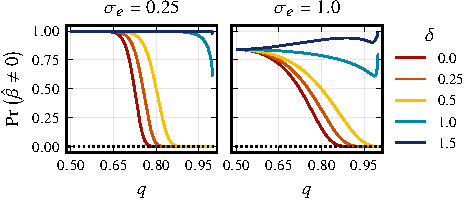
\includegraphics[]{plots/selection_probability.pdf}
  \caption{%
    Probability of selection in the lasso given a measurement noise level \(\sigma_\varepsilon\), a regularization parameter \(\lambda_1\), and a class balance \(q\). The scaling factor is parameterized by \(s_j = (q - q^2)^\delta\), \(\delta \geq 0\). The dotted line represents the asymptotic limit for the standardization case, \(\delta = 1/2\).}
  \label{fig:selection-probability}
\end{figure}

Now we turn to the impact of class imbalance on bias and variance of the elastic net estimator. We begin, in \Cref{thm:classbalance-bias}, by considering the expected value of the elastic net estimator in the limit as \(q \rightarrow 1^+\).

\begin{theorem}
  \label{thm:classbalance-bias}
  If \(\vec{x}_j\) is a binary feature with class balance \(q \in (0, 1)\), \(\lambda_1 \in (0,\infty)\), \(\lambda_2 \in [0,\infty)\), \(\sigma_\varepsilon > 0\), and \(s_j = (q - q^2)^{\delta}\), \(\delta \geq 0\)  then
  \[
    \lim_{q \rightarrow 1^+} \E \hat{\beta}_j =
    \begin{cases}
      0                                                                                                  & \text{if } 0 \leq \delta < \frac{1}{2}, \\
      \frac{2n \beta_j^*}{n + \lambda_2} \cdf\left(-\frac{\lambda_1}{\sigma_\varepsilon \sqrt{n}}\right) & \text{if } \delta = \frac{1}{2},        \\
      \beta^*_j                                                                                          & \text{if } \delta > \frac{1}{2}.
    \end{cases}
  \]
\end{theorem}

% \begin{remark}[Ridge Regression]
%   Asume the conditions of \Cref{thm:classbalance-bias} but that \(\lambda_1 = 0\). Then
%   \[
%     \lim_{q \rightarrow 1^+} \E \hat{\beta}_j =
%     \begin{cases}
%       0                                & \text{if } 0 \leq \delta < 1/2,     \\
%       \frac{n\beta_j^*}{n + \lambda_2} & \text{if } \delta = 1/2,            \\
%       \beta^*_j                        & \text{if } \delta \geq \frac{1}{2}.
%     \end{cases}
%   \]
% \end{remark}

\Cref{thm:classbalance-bias} shows that the bias of the elastic net estimator when \(0 \leq \delta < 1/2\) approaches
\(-\beta_j^*\) as \(q \rightarrow 1^+\). Interestingly, when \(\delta = 1/2\) (standardization), the estimate does not in fact tend to zero. Instead, it approaches the
true coefficient scaled by the probability that a standard normal variable is smaller than \(\beta_j^*\sqrt{n}\sigma_\varepsilon^{-1}\). For \(\delta > 1/2\), the
estimate is unbiased asymptotically, which is related to the scaled variance of the error term. Note that this unbiasedness is paralleled by a surge in variance and therefore also a rise in mean-squared error, and only serves to demonstrate that the cost of the decoupling of \(q\) is unbearable in the large noise--large imbalance scenario.
In \Cref{thm:classbalance-variance}, we continue by studying the variance in the limit as \(q \rightarrow 1^+\).

\begin{theorem}
  \label{thm:classbalance-variance}
  If \(\vec{x}_j\) is a binary feature with class balance \(q \in (0, 1)\) and \(\lambda_1,\lambda_2 \in (0,\infty)\), \(\sigma_\varepsilon > 0\), and \(s_j = (q - q^2)^{\delta}\), \(\delta \geq 0\), then
  \[
    \lim_{q \rightarrow 1^+} \var \hat{\beta}_j =
    \begin{cases}
      0      & \text{if } 0 \leq \delta < \frac{1}{2}, \\
      \infty & \text{if } \delta \geq \frac{1}{2}.
    \end{cases}
  \]
\end{theorem}

\begin{corollary}[Variance in Ridge Regression]
  \label{cor:ridge-variance}
  Assume the conditions of \Cref{thm:classbalance-variance} hold, except that \(\lambda_1 = 0\). Then
  \[
    \lim_{q \rightarrow 1^+} \var \hat{\beta}_j =
    \begin{cases}
      0                                          & \text{if } 0 \leq \delta < 1/4, \\
      \frac{\sigma_\varepsilon^2 n}{\lambda_2^2} & \text{if } \delta = 1/4,        \\
      \infty                                     & \text{if } \delta > 1/4.
    \end{cases}
  \]
\end{corollary}

\Cref{thm:classbalance-variance} formally proves the asymptotic variance effects of our scaling parameter \(s_j\) which we have already discussed in the context of selection probability and bias. Taken together with the results from \Cref{thm:classbalance-bias}, this suggests that the choice of scaling parameter, at least in the case of our specific parameterization, introduces a bias--variance tradeoff with respect to \(\delta\): to reduce bias (with respect to \(q\)), we need to pay the cost of increased variance.

In \Cref{fig:bias-var-onedim-lasso}, we now visualize bias, variance, and mean-squared error for ranges of class balance and various noise-level settings for a lasso problem. The figure demonstrates the bias--variance tradeoff that our asymptotic results suggested and indicates that the optimal choice of \(\delta\) is related to the noise level in the data. Since this level is unknown for most data sets, it suggests there might be value in selecting \(\delta\) through hyper-optimization as is typically done for the other hyper-parameters in the elastic net \((\lambda_1, \lambda_2)\)

\begin{figure}[htpb]
  \centering
  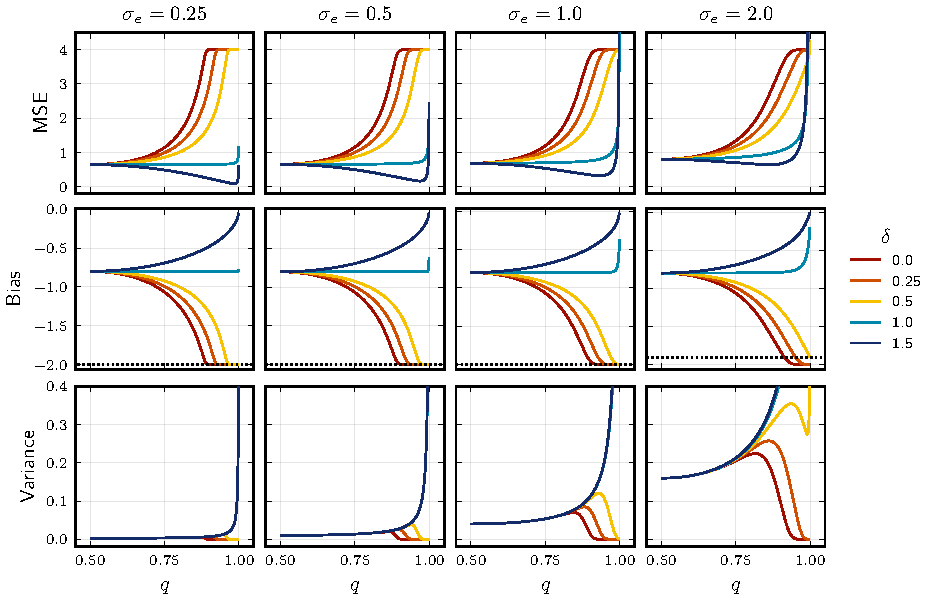
\includegraphics[]{plots/binary_onedim_bias_var_lasso.pdf}
  \caption{%
    Bias, variance, and mean-squared error for a one-dimensional lasso problem. We show these measures for various noise levels (\(\sigma_\varepsilon\)), class balances (\(q\)), and scaling factors (\(\delta\)).
    The dotted lines represent the asymptotic bias of the lasso estimator in the case of \(\delta = 1/2\).
  }
  \label{fig:bias-var-onedim-lasso}
\end{figure}

\begin{figure}[htpb]
  \centering
  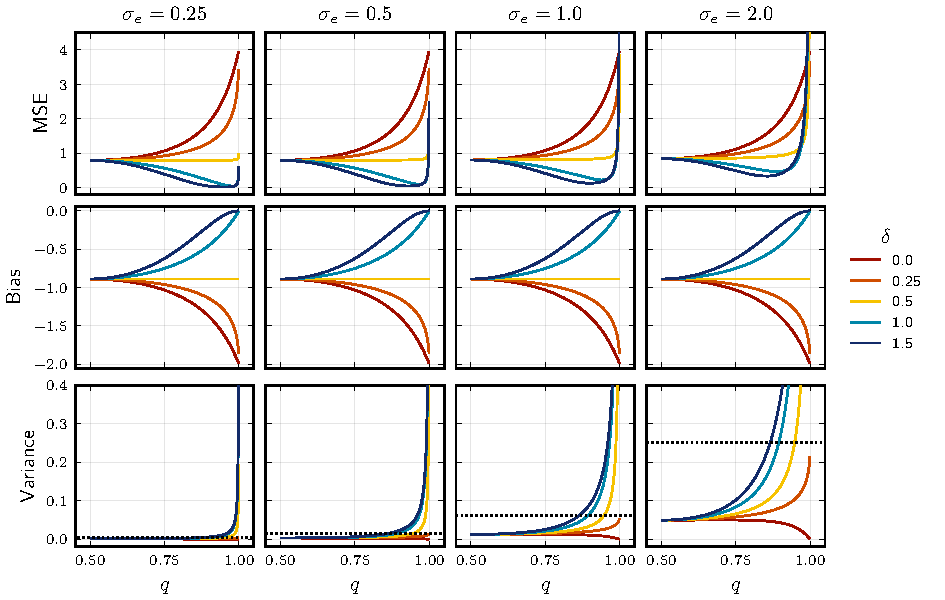
\includegraphics[]{plots/binary_onedim_bias_var_ridge.pdf}
  \caption{%
    Bias, variance, and mean-squared error for one-dimensional ridge regression. We show these measures for various noise levels (\(\sigma_\varepsilon\)), class balances (\(q\)), and scaling factors (\(\delta\)).
    The dotted lines represent the asymptotic bias of the lasso estimator in the case of \(\delta = 1/2\).
  }
  \label{fig:bias-var-onedim-ridge}
\end{figure}

So far, we have only considered a single binary feature. But under the assumption of orthogonal features, it is straightforward to introduce multiple binary features. In a first example, we study how the power of correctly detecting \(k=10\) signals under \(q\) linearly spaced in \([0.5, 0.99]\)~(\Cref{fig:binary-power}). We set \(\beta^*_j = 2\) for each of the signals, use \(n = 100\,000\), and let \(\sigma_\varepsilon = 1\). The level of regularization is set to \(\lambda_1 = n 4^\delta/10\). As we can see, the power is directly related to \(q\) and for unbalanced features stronger the higher the choice of \(\delta\) is.

We also consider a version of the same setup, but with \(p\) linearly spaced in \([20, 100]\) to compute the normalized mean-squared error (NMSE) and false discovery rate (FDR)~(\Cref{fig:binary-fdr-mse}). As before, we let \(k = 10\) and consider three different levels of class imbalance. The remaining \(p-k\) features have class balances spaced evenly on a logarithmic scale from 0.5 to 0.99. Unsurprisingly, the increase in power gained from selecting \(\delta = 1\) imposes increased false discovery rates. The mean-squared error depends on the class balance. For class-balanced signals, \(\delta \in \{0, 1/2\}\) proves to b the best choice, while for unbalanced signals, \(\delta = 1\) is the best choice. In the case when \(q = 0.99\), the model under scaling with \(\delta = 0\) is altogether unable to detect any of the true signals, instead picking up on the noisy, but better-balanced, features.

\begin{figure}[htpb]
  \centering
  \subcaptionbox{%
    The power (probability of detecting all true signals) of the lasso.
    In our orthogonal setting, power is constant over \(p\), which is why we have omitted the parameter in the plot.
    \label{fig:binary-power}
  }{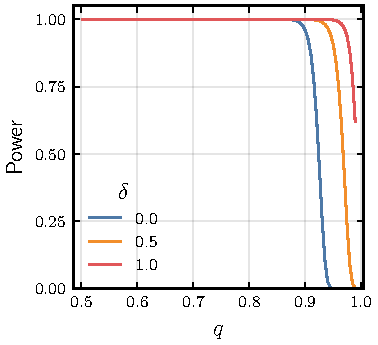
\includegraphics[]{plots/power.pdf}}\hfill%
  \subcaptionbox{%
    NMSE and FDR: the rate of coefficients incorrectly set to non-zero (false discoveries) to the total number of estimated coefficients that are nonzero (discoveries).
    \label{fig:binary-fdr-mse}
  }{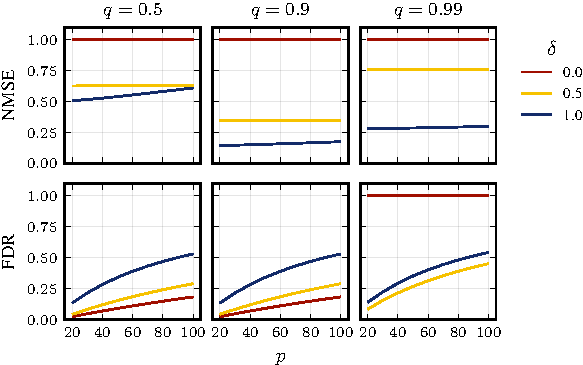
\includegraphics[]{plots/fdr_mse.pdf}}
  % 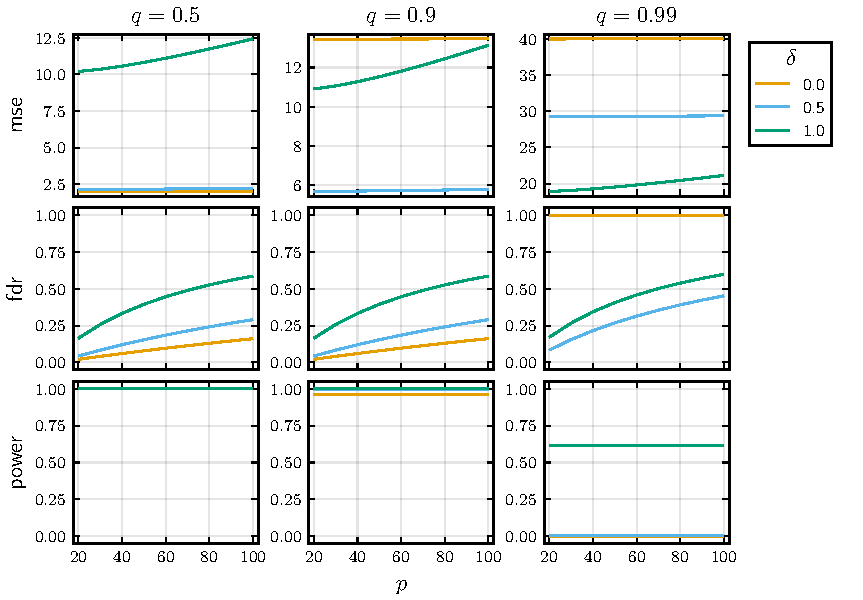
\includegraphics[]{plots/beta-bias-multidim.pdf}
  \caption{%
    Normalized mean-squared error (NMSE), false discovery rate (FDR), and power for a lasso problem with
    \(k = 10\) true signals (nonzero \(\beta_j^*\)), varying \(p\), and \(q \in [0.5, 0.99]\). The noise level is set at \(\sigma_\varepsilon = 1\) and \(\lambda_1 = 0.02\).
  }
  \label{fig:mse-fdr-power-binary}
\end{figure}

In \Cref{sec:experiments}, we will continue to study binary features in simulated experiments. For now, however, we will turn to the case of mixed data.

\subsection{Mixed Data}\label{sec:mixed-data}

In this section, we consider the case where the features are made up of a mix of continuous and and binary features.
Throughout the section, we will continue to assume that \(\mat{X}\) is fixed and that the features are orthogonal to one another.
As in our theoretical results, we will also restrict our focus to the case where the continuous features are normally distributed.

A fundamental problem in the context of mixed data is how to put the binary and normal features on the same scale, which we need to do in order for regularization to be, roughly speaking, ``fair'', given that the solution is sensitive to the scale of the features.
In essence, we need to say something about how an effect associated with a one-unit change in the binary feature (a flip) relates to a one-unit change in the continuous feature.
Since we assume our continuous feature to be normal, however, we will instead reason about change in terms of standard deviations of the normal feature.

To setup this situation more formally, we will say that the effect of a binary feature \(\vec{x}_1\) and a normal feature \(\vec{x}_2\) are \emph{comparable} if
\[
  \beta^*_1 = \kappa \sigma_{2}\beta^*_2,
\]
where \(\sigma_2\) is the standard deviation of \(\vec{x}_2\) and \(\kappa > 0\) is a scaling factor that represents the number of standard deviations (of the continuous feature) we consider achieves comparability between the features' effects. (Note that \(\sigma_2 \beta_2^*\) is just the standardized coefficient for the normal feature.) We illustrate this notion of comparability by a couple of examples.

\begin{example}
  Assume \(\kappa = 2\). If \(\vec{x}_2\) is sampled from \(\normal(\mu, 1/2^2)\), then the effects of \(\vec{x}_1\) and \(\vec{x}_2\) are comparable if \(\beta_1^* = \beta_2^*\).
\end{example}
\begin{example}
  Assume \(\kappa = 1\). If \(\vec{x}_2\) is sampled from \(\normal(\mu, 2^2)\), then the effects of \(\vec{x}_1\) and \(\vec{x}_2\) are comparable if \(\beta_1^* = 2\beta_2^*\).
\end{example}

Note that this definition refers to the data-generating mechanism, and not the regularized estimates.
What we ultimately want for comparability, however, is for the following relationship to hold:
\[
  \hat{\beta}_1 = \kappa \sigma_{2}\hat{\beta}_2.
\]
Put plainly, we want the effects of regularization to be distributed evenly across the estimates.
The crux of the problem is how to choose the scaling factor \(s_j\) for the binary features in order to achieve this effect for a given \(\kappa\).
Let us assume that we have two features, \(\vec{x}_1\) and \(\vec{x}_2\), where \(\vec{x}_1\) is binary and \(\vec{x}_2\) is normally distributed and that their effects are comparable in the sense given above.
Then it should hold that
\begin{alignat}{3}
  \label{eq:comparable-effects}
  \hat{\beta}_1                                                                                                                          & = \kappa \sigma_2\hat{\beta}_2                                                                                                                           & \implies \nonumber \\
  \frac{\st_{\lambda_1}(\tilde{\vec{x}}_1^\intercal \vec{y})}{s_1\left(\tilde{\vec{x}}_1^\intercal \tilde{\vec{x}}_1 + \lambda_2\right)} & = \frac{\kappa \sigma_2 \st_{\lambda_1}(\tilde{\vec{x}}_2^\intercal \vec{y})}{s_2\left(\tilde{\vec{x}}_2^\intercal \tilde{\vec{x}}_2 + \lambda_2\right)} & \implies \nonumber \\
  \frac{\st_{\lambda_1}\left(\frac{n\beta_1^* (q - q^2)}{s_1}\right)}{s_1\left(\frac{n(q - q^2)}{s_1^2} + \lambda_2\right)}              & = \frac{\kappa \st_{\lambda_1}\left(\frac{n\beta_1^*}{\kappa} \right)}{n + \lambda_2}
\end{alignat}
since we standardize he normal feature and therefore \(s_2 = \sigma_2\).
% First observe that there is no simple function \(s_j\) for which \Cref{eq:comparable-effects} holds in general (\(q \in [0, 1]\), \(\lambda_1,\lambda_2 \in \mathbb{R}^+\)). 
For the lasso (\(\lambda_2 = 0\)) and ridge regression (\(\lambda_1=0\)), we observe that \(s_1 = \kappa (q - q^2)\) and \(s_1 = (q - q^2)^{1/2}\), respectively, are the values for which \Cref{eq:comparable-effects} hold.
In other words, we can achieve comparability in the lasso by scaling each binary feature with its variance times \(\kappa\), the number of standard deviations we consider achieves comparability between the features' effects.
And for ridge regression, we can achieve comparability by scaling with standard deviation, irrespective of \(\kappa\).

% For other choices of \(\lambda_1\), \(\lambda_2\), and \(\delta\), we can only achieve comparability for a specific level of class balance, and never for \(\lambda_1 >0\), \(\lambda_2 >0\).
For any other choices of \(s_1\), equality can only hold for a specific level of class balance. If we let this level be \(q_0\), then, to achieve equality for \(\lambda_2 = 0\), we need \(s_1 =\kappa (q_0 - q_0^2)^{1 - \delta}(q - q^2)^\delta\). Similarly, for \(\lambda_1 = 0\), we need \(s_1 = (q_0 - q_0^2)^{1 - 2\delta} (q - q^2)^\delta\). In the sequel, we will assume that \(q_0 = 1/2\), to have effects be equivalent for the class-balanced case.

Note that this also means that there is an implicit relationship between the strength of penalization for binary and normal features, which depends on the level of class balance and normalization type. This means, for instance, that even in the class-balanced case (\(q = 1/2\)), we have to account for the type of normalization if we want binary and normal features to be treated equally. For example, if we were to use \(\delta=0\) and fit the lasso, then \Cref{eq:comparable-effects} for a binary feature with \(q=1/2\) becomes
\[
  \frac{4\st_{\lambda_1}\left(\frac{n\beta_1^*}{4}\right)}{n}               = \frac{\kappa \st_{\lambda_1}\left(\frac{n\beta_1^*}{\kappa} \right)}{n},
\]
which then implies \(\kappa = 4\), which may or may not agree with our assumptions about comparability between these features' effects.

For the rest of this paper, we will use \(\kappa = 2\). That is, we will say that the effects are comparable if the effect of a flip in the binary feature equals the effect of a two-standard deviation change in the normal feature. We base this argument on the discussion by \citet{gelman2008}, who argues that the classical approach of comparing standardized coefficients\footnote{Coefficients multiplied by the standard deviation of the respective feature.} awards effects of continuous features undue strength for most real data, since a change from, for instance, the lower to the upper 16\% of the distribution will equal approximately twice the effect of a change in the binary feature. Using two standard deviations as a comparability factor would, in contrast, equivocate this change with the flip of the binary feature, which we believe is a better default.
We want to stress that the choice of \(\kappa\) should, if possible, in general be made on a case-by-case (feature-by-feature) basis, using all available knowledge about the data at hand. But, irrespective of this, we also want to emphasize that the choice should be made. If you do not make it explicitly, then it will be implicitly dictated through the combination of normalization and penalization types you use.

Finally, note that the reasoning of comparability above rests on the assumption of no noise.
And we are, in fact, in general instead more interested in the expected value of the estimators, which depend on the noise level. In the case of large class-imbalances and large noise, for instance, our previous results (see \Cref{fig:bias-var-onedim-lasso} for instance), suggest that the estimators for normally distributed and binary features will not be comparable in this case.

% TODO: Say something about over and undersampling.

